\documentclass[twocolumn]{jarticle}

\usepackage{proceeding}
\usepackage{float}
\usepackage{enumitem}

\begin{document}

\pagestyle{empty}

\date{}
\title{大規模言語モデルを用いたなりすましプログラムの判定}
\author{高橋 琉生}
\maketitle

%% 現在ページの上部へのフロートの配置を抑制.
%% ここに記述しておくことで,最初のページの左段上部に図表を置かない.
\suppressfloats[t]


%%●●●●●●●●●●●●●●●
\section{まえがき}

プログラミングのソースコードの特徴分析に関する先行研究では,
大野ら\cite{lit:大野}がソースコードから得られる特徴を確率モデルで抽出し,そのモデルに学習させることで執筆者の識別などに応用している.
一方で,ChatGPTなどの大規模言語モデル(Large Language Model, 以下LLM)が急速に普及したことにより,
ソースコードを人間自身が書かない状況が増えている.
この現象は,研究や学習の現場においても,ソースコードの真正性や執筆者の特定に新たな課題をもたらしている.

本研究では,このような状況を踏まえ,ソースコードの執筆者固有の癖をLLMで捉えるアプローチを検討する.
具体的には,Chain-of-Thought(以下CoT)\cite{lit:Jason}を用いて,
対象者によって作成された複数のソースコードをLLMに入力し,その表現パターンを学習させることで,
対象者自身が執筆したかどうかを判定する枠組みを構築することを目的とする.
本手法は,コード生成AIの普及による執筆者の同定の難しさに対して,有効な解決策となり得る可能性があると考えられる.

%%●●●●●●●●●●●●●●●
\section{なりすまし判定システム}
本研究では,対象者(人間)が書いたソースコードか,
LLMによって生成されたなりすましのソースコードを判定することを目的とする.
対象者のコーディングスタイルを真似てソースコードを生成するLLMを``なりすましLLM"と呼ぶことにする.
判定もLLMによって行い,これを``判定LLM"と呼ぶことにする.

実験の概略を説明する.対象者にC言語の問題を与え,ソースコードを10個作成してもらう.
一方,なりすましのソースコードは,なりすましLLMに対象者が書いたソースコードの5つを与え,
対象者のコーディングスタイルを記憶させる.
判定実験では,判定LLMに対象者が書いたソースコードとなりすましのソースコードのいずれかを与え,判定させる.
本研究では,対象者(人間)を1名に限定した.

\section{実験方法}

\subsection{ChatGPT 4o}
本研究のLLMはChatGPT 4oを使用した.
% ChatGPTを使用した理由を図などを使用して論理的に説明する
% パラメータの数など
ChatGPT 4oは,具体的なパラメータ数は公開されていないものの,
HELM\cite{lit:Percy,lit:helm}によるとMean win rateが最も高いので,
本研究ではChatGPT 4oを用いる.

\subsection{CoTでプログラムの特徴分析方法を与える}

\begin{figure}%[H]
	\begin{center}
	 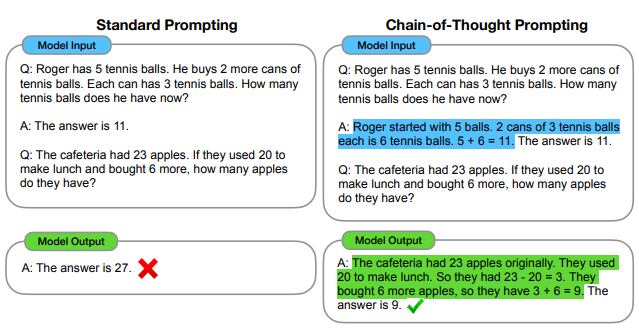
\includegraphics[scale=0.6]{chain_of_thought_fig_1.png}
	 \caption{Chain-of-Thought}
	 \label{fig:chain_of_thought}
	\end{center}
 \end{figure}

図\ref{fig:chain_of_thought}のように,
ユーザーの質問を最初にプロンプトに与えるのではなく,考え方を与えLLM自身に考えさせる.
ソースコードの評価項目は以下のように設定した.
% ChatGPTに質問したって書く?

\begin{enumerate}
	\setlength{\parskip}{0cm} % 段落間
	\setlength{\itemsep}{0cm} % 項目間
	\item コーディングスタイル・フォーマット
	\item コメントやドキュメンテーションの特徴
	\item コード設計上の特徴
	\item 構文・言語機能の利用傾向
	\item コードの正確性
	\item 上記以外の特筆すべき特徴
\end{enumerate}

\subsection{対象者のソースコードの特徴}

本研究で使用した対象者のソースコードの特徴について述べる.
(1)コーディングスタイルは空行とスペースが多いK&Rスタイルであった.
(2)変数名は短く,直感的な命名方法であった.
(3)コメントは存在しなかった.
(4)実行結果出力は簡潔であった.
(5)関数分割や標準ライブラリは時々使用している.

\subsection{なりすましLLM(学習あり)}

先ほど述べた特徴を持つなりすましLLMである.
学習ありでは,CoTで特徴を学習させて,対象者の特徴を持つソースコードを生成させた.
コメントアウトは無く,変数名も対象者のソースコードと類似して直感的で短くなっている.

\subsection{なりすましLLM(学習なし)}

Zero-shot Promptingでは,回答例を与えず,問題だけを与え,ソースコードを生成させた.
この生成されたソースコードにはコメントアウトが適切に記述されている.
ChatGPTは指示がなくともコメントアウトを記述してくれる.

\section{実験結果}

対象者となりすましのソースコードを判定できれば正解とする.
正解率は出題した問題に対する正解の割合を指す.

なりすましのソースコードを対象者のソースコードと判定した場合,偽陽性とする.
一方で,偽陰性は対象者のソースコードをなりすましのソースコードと判定した場合のことを指す.
偽陽性率は出題したなりすましのソースコードに対する偽陽性の割合を指す.
偽陰性率は出題した対象者のソースコードに対する偽陰性の割合を指す.

ChatGPTの判定は確率的な挙動を示すため,判定結果が常に同じとは限らずゆらぎがある.
そのため,1回の判定あたりソースコードを5個出題し,10回繰り返す.
さらに,学習用と判定用のソースコードをそれぞれ5種類用意し,全体で250個出題した.
対象者のソースコードとなりすましのソースコードはそれぞれ125個ずつ出題した.



\subsection{なりすましLLM(学習あり)}

% 表1 なりすまし(学習あり)の正解率
\begin{table}%[H]
	\begin{center}
		\caption{なりすましLLM(学習あり)の正解率}
		\label{tbl:spoofing}
	\begin{tabular}{lrrr} \hline
		  & 正解率(\%) & 偽陽性率(\%) & 偽陰性率(\%)  \\ \hline
	  1 &      42.0 &         96.7 &         0.0  \\
		2 &      48.0 &         85.0 &        30.0  \\ 
	  3 &      56.0 &         86.7 &        25.7  \\ 
	  4 &      34.0 &         82.3 &        26.7  \\ 
	  5 &      24.0 &        100.0 &        52.0  \\ \hline
	合計 &     40.8 &         90.4 &        28.0  \\ \hline
\end{tabular}
	\end{center}
\end{table}


結果は表\ref{tbl:spoofing}のようになった.
表\ref{tbl:spoofing}は想定していた結果になり,
正解率が平均40%と低く,偽陽性率も90%と高いため,
なりすましLLMを見破れていないことが分かる.

\subsection{なりすましLLM(学習なし)}

% 表2 なりすましLLM(学習なし)の正解率
\begin{table}%[H]
	\begin{center}
		\caption{なりすましLLM(学習なし)の正解率}
		\label{tbl:Zero-shot}
	\begin{tabular}{lrrr} \hline
			& 正解率(\%) & 偽陽性率(\%) & 偽陰性率(\%)  \\ \hline
		1 &      66.0 &         33.3 &        35.0  \\
		2 &      72.0 &         50.0 &        13.3  \\ 
		3 &      72.0 &         40.0 &        22.9  \\ 
		4 &      70.0 &         40.0 &         6.7  \\ 
		5 &      36.0 &         88.0 &        40.0  \\ \hline
	合計 &     63.2 &        	 49.6 &        24.0  \\ \hline
\end{tabular}
	\end{center}
\end{table}


結果は表\ref{tbl:Zero-shot}のようになった.
正解率は表\ref{tbl:spoofing}と比較して上昇し,60%~70%と概ね正解できているが,
想定していた目標値80%より低い値になってしまった.
さらに,与えるソースコードによっては正解率50%を割ってしまうこともあった.
学習させたソースコードはライブラリを使用していたが,
出題したソースコードでは使っていないとChatGPTは判定したことが原因だと考えられる.


%%●●●●●●●●●●●●●●●
\section{まとめ}
% 段落を意識.まとめるなら段落1つにつき結論を1つ用意する
% 何が言いたいかを書く

本研究はなりすましLLMの学習ありと学習なしの2種類を用意して現状のLLMの特徴分析能力を探った.
実験では可能性を示したものの,精度が問題である.

学習なしの場合では60%程度判定できているが,目標値に到達していない.
これはChatGPTの記憶できる限界以上のトークンを与えたことが原因だと考えられる.
学習なしのソースコードはコメントがあるにもかかわらず,判定時には「コメントなし」と判断され,対象者のものだと誤判定される場合があった.

また,原因の1つとして学習させるサンプルが少なすぎることが挙げられる.
サンプルが少ないと,対象者のコーディングスタイル全体を適切に推測できないと考えられる.
例えば,関数分割やmallocによる動的確保は必ず行うわけではないので,
サンプルにない特徴を与えてしまうとなりすましだと判定してしまう.
しかし,対象者と確証できるソースコードを大量に用意する必要があるので,
サンプルソースコードが少なくても特徴を分析できる手法を考察する必要がある.

他にも,執筆者が同じでも,対象者のスキルアップの影響でコーディングスタイルが変化することがある.
ゆえに,判定LLMに学習させるソースコードと判定させるソースコードは同時期に執筆されていることが必須である.

今後の課題として,偽陰性率を0%に抑えながら,偽陽性率を低減することが求められる.
そのために,今後の研究では以下のアプローチを試みる予定である.
\begin{itemize}
	\setlength{\parskip}{0cm} % 段落間
	\setlength{\itemsep}{0cm} % 項目間
  \item Self-Consistency\cite{lit:Xuezhi}やScore-Anchoringなどの別のプロンプト手法を試す.
  \item より高度な推論能力を持つChatGPT o1や,よりコンテキスト保持能力をもつclaudeなど,別のLLMを用いる.
  \item C++やPythonなど他のプログラミング言語を用いた検証.
  %\item 別の対象者の場合でも対応.
  \item AtCoderのデータを利用したさらなる分析.
\end{itemize}
最終的には,対象者となりすましのソースコードを正しく判定できるシステムを構築したいと考えている.

\begin{thebibliography}{9}
 \renewcommand{\baselinestretch}{1.0}
 \small

 \bibitem{lit:大野}
	大野 麻子, 村尾 元.
 	``確率モデルによるソースコード記述スタイルの識別'',
	 第53回システム制御情報学会研究発表講演会,2009.

 \bibitem{lit:Jason}
   Jason Wei,et al.
	 ``Chain-of-Thought Prompting Elicits Reasoning in Large Language Models'',
	 arXiv,arXiv:2201.11903,2022.

 \bibitem{lit:Percy}
  Percy Liang,et al.
	 ``Holistic Evaluation of Language Models',
	 arXiv,arXiv:2211.09110,2022. 

 \bibitem{lit:helm}
	 ``Holistic Evaluation of Language Models (HELM)'',
	 \verb|https://crfm.stanford.edu/helm/lite/latest/|

 \bibitem{lit:Xuezhi}
	 Xuezhi Wang,et al.
	 ``Self-Consistency Improves Chain of Thought Reasoning in Language Models'',
	 arXiv,arXiv:2203.11171,2022.

\end{thebibliography}

\end{document}

